% Level ceiling (grade 8): powers of ten written in math mode as
% $3 \times 10^8$ (math g8-03); NO \qty e-notation and no formal
% scientific-notation machinery (both arrive in grade 9).
\chapter{Kelajuan Cahaya; Jarak di Alam Semesta}\label{ch:g8:speed-of-light}

Selama tujuh tahun buku ini berbisik bahwa \omterm{def:g1:light-and-shadows:source}{cahaya} ``sama saja dengan
seketika'' --- kilat sebelum guruhnya, benturan yang terlihat yang
memulai stopwatchnya. Bab ini menepati janji keluarganya yang tertua:
\omterm{def:g7:motion-average-speed:formula}{kelajuan} \omterm{def:g1:light-and-shadows:source}{cahaya} tidak tak terhingga, manusia \omterm{def:g6:measurement-in-science:measuring}{mengukurnya} walau
peluangnya kecil, dan bilangannya begitu luas sehingga ia menjadi,
dalam satu tarikan napas, penggaris ilmu falak sekaligus mesin
waktunya.

\section{Pengukuran yang mustahil}

\begin{example}[Lentera di atas dua bukit]\label{ex:g8:speed-of-light:galileo}
Empat abad yang lalu, perintis besar percobaan menempatkan dua
pengamat di atas bukit yang berjauhan pada malam hari, masing-masing
dengan lentera bertutup: bukalah tutupmu begitu melihat tutupku
terbuka, dan kelambatan pulang perginya seharusnya mengkhianati
\omterm{def:g7:motion-average-speed:formula}{kelajuan} \omterm{def:g1:light-and-shadows:source}{cahaya}. Kelambatan yang mereka temukan hanyalah waktu tanggap
manusia; di antara kedua bukitnya, penyeberangan \omterm{def:g1:light-and-shadows:source}{cahaya} yang
sesungguhnya memakan beberapa \emph{perjutaan} sekon. Percobaannya
gagal dengan gemilang --- setidaknya membuktikan bahwa \omterm{def:g1:light-and-shadows:source}{cahaya} lebih
cepat daripada apa pun yang dapat dicatat waktunya dari puncak bukit,
lalu menantang ilmu falak mencari \omterm{def:g6:describing-motion:trajectory}{lintasan} balap yang lebih panjang.
\end{example}

\begin{example}[Bulan yang datang terlambat]\label{ex:g8:speed-of-light:romer}
\omterm{def:g6:describing-motion:trajectory}{Lintasan} balapnya datang atas kebaikan Jupiter. \omterm{def:g2:moon-in-the-sky:moon}{Bulan} besarnya yang
paling dalam tergerhana masuk ke \omterm{def:g1:light-and-shadows:shadow}{bayang-bayang} Jupiter menurut jadwal
yang teramat teratur --- sebuah \omterm{ex:g2:measuring-time:clock}{jam} di langit. Namun seorang ahli
falak yang sabar menemukan \omterm{ex:g2:measuring-time:clock}{jamnya} berjalan \emph{terlambat} sampai
beberapa menit pada bulan-bulan ketika \omterm{def:g6:sun-earth-moon:axisorbit}{orbit} Bumi telah membawa kita
ke sisi Matahari yang jauh dari Jupiter, lalu lebih awal lagi ketika
kita berayun mendekat. Lompatannya: bulannya tepat waktu ---
\emph{\omterm{def:g1:light-and-shadows:source}{cahayanya}} yang tertunda, karena memerlukan waktu tambahan untuk
menyeberangi lebar tambahan \omterm{def:g6:sun-earth-moon:axisorbit}{orbit} Bumi. Dari keterlambatannya dan
ukuran \omterm{def:g6:sun-earth-moon:axisorbit}{orbitnya} datanglah taksiran \omterm{def:g7:motion-average-speed:formula}{kelajuan} \omterm{def:g1:light-and-shadows:source}{cahaya} yang pertama ---
sangat dekat dengan kebenarannya, untuk ukuran abad ketujuh belas.
\end{example}

\begin{omfigure}
\begin{tikzpicture}[scale=0.8]
  \fill[omThm] (4.6,1.7) circle (0.42);
  \node[below, font=\small] at (4.6,1.1) {Matahari};
  \draw[dashed, omExo] (4.6,1.7) ellipse (2.6 and 1.05);
  \fill[omDef] (2.0,1.7) circle (0.18);
  \node[below, font=\footnotesize] at (2.0,1.3) {Bumi, dekat};
  \fill[omDef, opacity=0.5] (7.2,1.7) circle (0.18);
  \node[below, font=\footnotesize] at (7.5,1.3) {Bumi, jauh};
  \fill[omExo] (0.6,1.7) circle (0.3);
  \node[above, font=\small] at (0.6,2.1) {Jupiter dan bulannya};
  \draw[-Stealth, omThm, thick] (0.95,1.78) -- (1.8,1.74);
  \draw[-Stealth, omThm, thick] (0.95,1.62) -- (7.0,1.64);
  \node[below, font=\footnotesize, omThm] at (5.2,0.35)
    {cahaya dari kedudukan yang jauh menyeberangi seluruh orbitnya sebagai tambahan};
\end{tikzpicture}

{\small \omterm{def:g2:moon-in-the-sky:moon}{Bulan} yang datang terlambat: berita gerhana dari Jupiter
mencapai Bumi di sisi yang jauh beberapa menit di belakang jadwalnya
--- kelambatannya adalah \omterm{def:g1:light-and-shadows:source}{cahaya}, tertangkap sedang bepergian.}
\end{omfigure}

\begin{proposition}[Kelajuan cahaya]\label{prop:g8:speed-of-light:value}
Di dalam hampa \omterm{def:g2:air-around-us:air}{udara} --- dan di dalam \omterm{def:g2:air-around-us:air}{udara}, dengan hampiran yang
sangat baik --- \omterm{def:g1:light-and-shadows:source}{cahaya} berjalan pada
\[
c = \qty{300000}{km/s} = 3 \times 10^{8}\ \unit{m/s},
\]
tiga ratus ribu kilometer tiap sekon: tujuh setengah putaran
mengelilingi Bumi di antara dua denyut jantung. Setiap warna
campurannya berjalan pada $c$ yang sama ini di dalam hampa \omterm{def:g2:air-around-us:air}{udara};
tidak ada yang membawa materi atau berita yang pernah tercatat lebih
cepat. Kemudian, kecerdikan di Bumi menegaskan para ahli falak ---
sebuah \omterm{def:g6:light-propagation:ray}{berkas} yang dicincang roda bergigi yang berputar, berlomba
delapan kilometer ke sebuah \omterm{def:g5:mirrors-reflection:reflection}{cermin} lalu kembali menembus celah gigi
berikutnya --- dan alat zaman sekarang telah memoles $c$ sampai ke
kepastian yang begitu lengkap sehingga \omterm{def:g2:measuring-length:units}{meternya} sendiri kini
dibatasi darinya.
\end{proposition}

\begin{example}[Waktu tempuh di sekitar kita]\label{ex:g8:speed-of-light:times}
Dengan $t = d/c$, \omterm{def:g4:solar-system:family}{Tata Surya} memperoleh sebuah jadwal. \omterm{def:g2:moon-in-the-sky:moon}{Bulan},
\qty{384000}{km}: $384000 \div 300000 \approx
\qty{1.3}{s}$ --- percakapan radio Bumi--Bulan membawa jeda yang
canggung itu. Matahari, $150$ juta km: $150000000 \div
300000 = \qty{500}{s}$ --- delapan menit dua puluh: sinar matahari
selalu berupa berita berumur delapan menit. Mars, pada jarak khas $2 \times
10^{8}$ km: kira-kira sebelas menit --- para pengemudi penjelajahnya
mengirim rencana hari itu lalu menunggu; tidak ada \omterm{def:g3:levers-and-scales:lever}{tuas} kendali yang
dapat mengemudi menyeberangi perjalanan pulang pergi dua puluh menit.
\end{example}

\begin{omfigure}
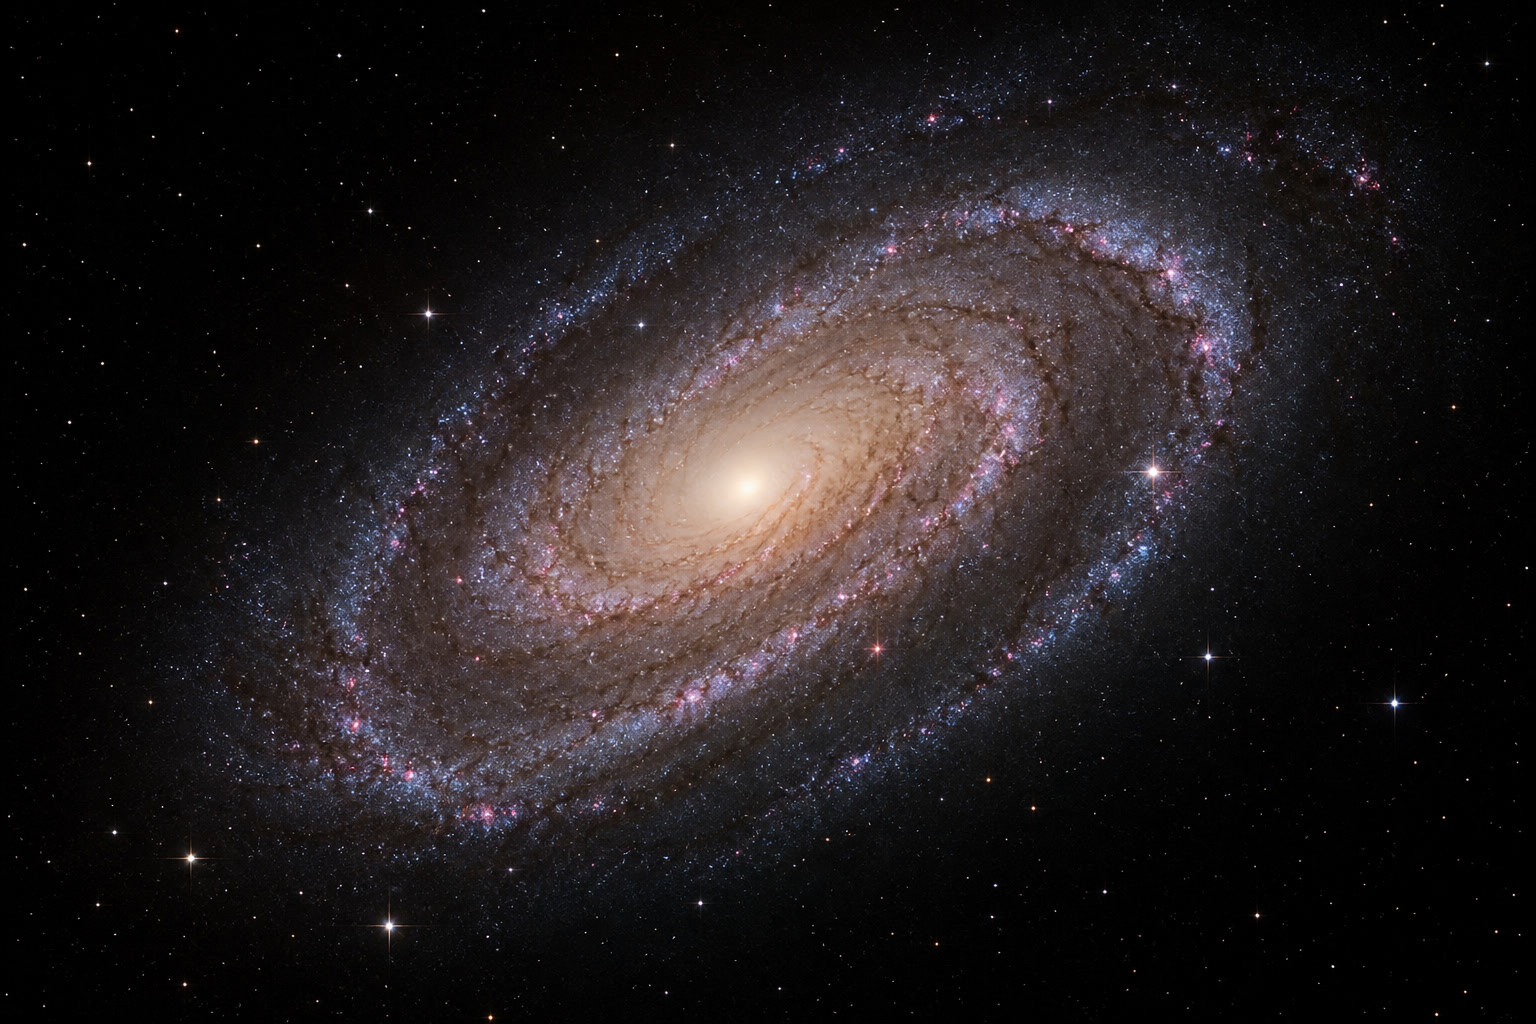
\includegraphics[width=0.55\linewidth]{images/book1/ai/g8-universe-galaxy.jpg}

{\small Sebuah galaksi berpilin: \omterm{def:g1:light-and-shadows:source}{cahaya} dari \omterm{def:g4:solar-system:star}{bintangnya} menyeberangi antariksa kosong berjuta-juta tahun sebelum mencapai teleskop mana pun.}
\end{omfigure}

\section{Tahun cahaya}

\begin{definition}[Tahun cahaya]\label{def:g8:speed-of-light:lightyear}
Sebuah \emph{tahun cahaya}\index{tahun cahaya} adalah sebuah
\emph{jarak}: bentangan yang ditempuh \omterm{def:g1:light-and-shadows:source}{cahaya} dalam satu tahun ---
kira-kira $9.5 \times
10^{12}$ km, hampir sepuluh juta juta kilometer. Namanya menyesatkan
yang tergesa-gesa (ia bukan waktu, sebagaimana ``langkah kaki'' bukan
kaki); ahli falak memakainya karena kilometer runtuh di bawah skala
langit yang sesungguhnya.
\end{definition}

\begin{example}[Sekitar kita dalam tahun cahaya]\label{ex:g8:speed-of-light:ladder}
\omterm{def:g4:solar-system:star}{Bintang} terdekat di luar Matahari: kira-kira $4$ \omterm{def:g8:speed-of-light:lightyear}{tahun cahaya} ---
\omterm{def:g1:light-and-shadows:source}{cahaya} malam ini meninggalkannya ketika kamu masih di bab fisikamu
yang pertama. \omterm{def:g4:solar-system:star}{Bintang} terang langit \omterm{def:g3:sun-days-seasons:year}{musim} dingin: puluhan sampai
ratusan \omterm{def:g8:speed-of-light:lightyear}{tahun cahaya}. \omterm{ex:g5:stars-night-sky:milkyway}{Bima Sakti}, kota \omterm{def:g4:solar-system:star}{bintang} kita: kira-kira
$100000$ \omterm{def:g8:speed-of-light:lightyear}{tahun cahaya} lebarnya. Galaksi tetangga besar yang terdekat:
kira-kira $2.5$ juta \omterm{def:g8:speed-of-light:lightyear}{tahun cahaya} --- nodanya yang samar, yang
terlihat oleh mata telanjang yang sudah menyesuaikan diri dengan
gelap, adalah \omterm{def:g1:light-and-shadows:source}{cahaya} tertua yang dapat dilihat manusia tanpa alat.
\end{example}

\begin{proposition}[Teleskop adalah mesin waktu]\label{prop:g8:speed-of-light:timemachine}
Karena berita \omterm{def:g1:light-and-shadows:source}{cahaya} berjalan pada $c$ dan alam semestanya luas,
\emph{memandang jauh berarti memandang mundur}. \omterm{def:g4:solar-system:star}{Bintang} pada $4$
\omterm{def:g8:speed-of-light:lightyear}{tahun cahaya} menunjukkan dirinya sebagaimana ia $4$ tahun yang lalu;
galaksi tetangganya, sebagaimana ia ketika nenek moyang kita pertama
kali menyerpih perkakas batu. Kecurigaan pengamat \omterm{def:g4:solar-system:star}{bintang} kelas lima
kini menjadi teorema hitungan: setiap teleskop yang dibidikkan ke luar
dibidikkan ke masa lalu, dan ilmu falak adalah sejarah yang dibaca
dengan \omterm{def:g1:light-and-shadows:source}{cahaya} \omterm{def:g4:solar-system:star}{bintang}.
\end{proposition}

\begin{method}[Mengubah jarak dan pandangan mundur]\label{met:g8:speed-of-light:convert}
\begin{enumerate}
  \item jarak dalam \omterm{def:g8:speed-of-light:lightyear}{tahun cahaya} $\to$ pandangan mundur dalam tahun:
        bilangan yang sama --- itulah seluruh kejeniusan \omterm{def:g6:measurement-in-science:measuring}{satuannya};
  \item jarak dalam kilometer $\to$ waktu \omterm{def:g1:light-and-shadows:source}{cahaya}: bagilah dengan
        \qty{300000}{km/s}, lalu jinakkan sekonnya menjadi menit,
        \omterm{ex:g2:measuring-time:clock}{jam}, atau tahun;
  \item \omterm{def:g8:speed-of-light:lightyear}{tahun cahaya} $\to$ kilometer (jarang berharga):
        kalikan dengan $9.5 \times 10^{12}$ --- lalu ingatlah
        mengapa ahli falak jarang melakukannya.
\end{enumerate}
\end{method}

\begin{remark}[Apa arti ``sekarang'' di sana]\label{rem:g8:speed-of-light:now}
Apakah \omterm{def:g4:solar-system:star}{bintang} empat \omterm{def:g8:speed-of-light:lightyear}{tahun cahaya} itu masih bersinar \emph{saat ini}?
Hampir pasti --- \omterm{def:g4:solar-system:star}{bintang} berumur panjang --- tetapi tidak ada jawaban
yang lebih cepat daripada \omterm{def:g1:light-and-shadows:source}{cahaya} sendiri yang pernah dapat mencapai
kita: berita yang sesegar mungkin sudah basi empat tahun, selalu.
Untuk langit yang dalam, pertanyaannya melunak menjadi keanehan:
sebagian noda yang paling samar di dalam teleskop besar adalah galaksi
yang \omterm{def:g1:light-and-shadows:source}{cahayanya} berangkat sebelum Bumi ada. Fisika akan mempertajam apa
yang bahkan dapat berarti ``sekarang pada jarak jauh'' pada
tahun-tahun perguruan tinggi; untuk tahun ini, bawalah versi yang
jujur: langit bukanlah sebuah pemandangan --- ia sebuah arsip.
\end{remark}

\section{Latihan}

\begin{exercise}[$\star$]\label{exo:g8:speed-of-light:1}
Berikan $c$ dalam \unit{km/s} dan dalam \unit{m/s} (dalam bentuk
pangkat sepuluh). Apa yang gagal di atas kedua bukitnya, dan mengapa?
\end{exercise}

\begin{exercise}[$\star$]\label{exo:g8:speed-of-light:2}
Ceritakan ulang hujah bulan yang terlambat itu dalam tiga kalimat: apa
yang tepat waktu, apa yang terlambat, dan apa yang diukur
keterlambatannya.
\end{exercise}

\begin{exercise}[$\star$]\label{exo:g8:speed-of-light:3}
Hitunglah waktu tempuh \omterm{def:g1:light-and-shadows:source}{cahaya}: \omterm{def:g2:moon-in-the-sky:moon}{Bulan} (\qty{384000}{km}); Matahari
($150$ juta km). Mengapa sinar matahari berupa ``berita basi''?
\end{exercise}

\begin{exercise}[$\star$]\label{exo:g8:speed-of-light:4}
Sebuah \omterm{def:g8:speed-of-light:lightyear}{tahun cahaya} --- waktu atau jarak? Batasilah, lalu berikan
ukurannya dalam kilometer (dalam bentuk pangkat sepuluh).
\end{exercise}

\begin{exercise}[$\star$]\label{exo:g8:speed-of-light:5}
\omterm{def:g4:solar-system:star}{Bintang} terdekat duduk kira-kira $4$ \omterm{def:g8:speed-of-light:lightyear}{tahun cahaya} jauhnya. Berapa
pandangan mundur malam ini --- dan kamu sedang melakukan apa ketika
\omterm{def:g1:light-and-shadows:source}{cahayanya} berangkat?
\end{exercise}

\begin{exercise}[$\star$]\label{exo:g8:speed-of-light:6}
Mengapa tidak seorang pun dapat mengendalikan penjelajah Mars dengan
\omterm{def:g3:levers-and-scales:lever}{tuas} kendali dari Bumi? Pakailah bilangan contoh jadwalnya.
\end{exercise}

\begin{exercise}[$\star$]\label{exo:g8:speed-of-light:7}
Urutkan menurut pandangan mundurnya: \omterm{def:g2:moon-in-the-sky:moon}{Bulan}; Matahari; \omterm{def:g4:solar-system:star}{bintang}
terdekat; galaksi tetangganya --- dengan angka kasar masing-masing.
\end{exercise}

\begin{exercise}[$\star$]\label{exo:g8:speed-of-light:8}
``\omterm{def:g2:measuring-length:units}{Meternya} kini dibatasi dari $c$.'' Apa yang dikatakan hal ini
tentang yang mana di antara keduanya --- penggaris atau \omterm{def:g1:light-and-shadows:source}{cahaya} ---
yang lebih dalam dipercaya para fisikawan?
\end{exercise}

\begin{exercise}[$\star\star$]\label{exo:g8:speed-of-light:9}
Penjarakan radar: sebuah denyut radio (yang berjalan pada $c$) yang
dipantulkan dari \omterm{def:g2:moon-in-the-sky:moon}{Bulan} kembali dalam kira-kira \qty{2.6}{s}. Pulihkan
jarak \omterm{def:g2:moon-in-the-sky:moon}{Bulan} dari perjalanan pulang pergi ini --- lalu sebutkan aturan
sonar lama yang berlaku pula di sini.
\end{exercise}

\begin{exercise}[$\star\star$]\label{exo:g8:speed-of-light:10}
Urutkan menurut kedalaman arsipnya: \omterm{def:g1:light-and-shadows:source}{cahaya} di dalam kamarmu dari
sebuah lampu (\qty{3}{m}); Matahari; sebuah \omterm{def:g4:solar-system:star}{bintang} pada $100$ \omterm{def:g8:speed-of-light:lightyear}{tahun
cahaya}; galaksi tetangganya. Untuk lampunya, taksirlah pandangan
mundurnya dalam permiliaran sekon ($3 \div (3 \times 10^{8})$ ---
jinakkan dengan kata-kata).
\end{exercise}

\begin{exercise}[$\star\star$]\label{exo:g8:speed-of-light:11}
Sebuah laporan berita berkata ``para ahli falak menonton sebuah
\omterm{def:g4:solar-system:star}{bintang} meledak Selasa lalu, $8000$ \omterm{def:g8:speed-of-light:lightyear}{tahun cahaya} jauhnya.'' Tulislah
ulang kalimatnya dengan keterangan waktu yang jujur: kapan ledakannya
terjadi, dan apa yang terjadi Selasa lalu?
\end{exercise}

\begin{exercise}[$\star\star\star$]\label{exo:g8:speed-of-light:12}
Keterlambatan bulan itu memuncak pada kira-kira $1000$ sekon ---
waktu \omterm{def:g1:light-and-shadows:source}{cahaya} untuk menyeberangi lebar penuh \omterm{def:g6:sun-earth-moon:axisorbit}{orbit} Bumi, kira-kira
$3 \times 10^{8}$ km. Jalankan sendiri pembagian abad ketujuh belas
itu lalu bandingkan dengan $c$ zaman sekarang: sejujur apa jawaban
pertama sang langit?
\end{exercise}

\section{Soal: Pusat Kendali Misi}

\begin{problem}[{Soal akhir pekan --- satu giliran jaga di pusat
kendali misi antariksa dalam; percakapan berkelambatan cahaya dari
Bulan sampai ke bintang; buku petunjuk
pengoperasiannya}]\label{pb:g8:speed-of-light:1}
Malam ini kamu memimpin meja komunikasinya: setiap pesan berjalan pada
$c = \qty{300000}{km/s}$, dan kelambatan \omterm{def:g1:light-and-shadows:source}{cahayanya} mengatur setiap
keputusan.

\medskip\noindent\textbf{Bagian I --- Pengoperasian yang dekat.}
\begin{enumerate}
  \item Pangkalan bulannya (\qty{384000}{km}) meminta penegasan
        penurunan bekal. Berapa lama sesudah ``ditegaskan''-mu
        pangkalannya mendengarnya, dan paling cepat kapan kamu dapat
        mendengar pengakuan penerimaan mereka?
  \item Sebuah satelit di \omterm{def:g6:sun-earth-moon:axisorbit}{orbit} tinggi pada \qty{36000}{km}
        meneruskan siaran televisi. Hitunglah kelambatan sekali
        jalannya --- lalu katakan mengapa panggilan telepon
        antarbenua lewat satelit semacam itu membawa keraguan yang
        baru saja terasa (pulang pergi naik dan turun).
  \item Observatorium mataharinya melaporkan suar besar ``ketika ia
        terjadi''. Betulkan ungkapan sang penjaganya: kapan suarnya
        sungguh meletus?
  \item Tata caranya meminta semua \omterm{ex:g2:measuring-time:clock}{jam} memberi kelonggaran bagi
        kelambatannya. Sambungan dekat-Bumi yang mana --- \omterm{def:g2:moon-in-the-sky:moon}{Bulan} atau
        satelit tinggi --- yang memerlukan kelonggaran yang lebih
        besar, dan kira-kira dengan faktor berapa?
\end{enumerate}

\medskip\noindent\textbf{Bagian II --- Jendela Marsnya.}
Mars berdiri malam ini pada $1.8 \times 10^{8}$ km.
\begin{enumerate}[resume]
  \item Hitunglah kelambatan sekali jalannya dalam sekon, lalu dalam
        menit.
  \item Penjelajahnya bertemu celah jurang yang tak terduga dan
        kameranya menunjukkannya mendekat pada langkah orang berjalan.
        Jelaskan, dengan angka pulang perginya, mengapa penyelamatan
        dengan \omterm{def:g3:levers-and-scales:lever}{tuas} kendali tidak ada harapannya --- dan karena itu
        apa yang harus dibawa penjelajahnya di dalam dirinya sendiri.
  \item Pengunggahan rencana malam itu memakan \qty{3}{min}
        pemancaran ditambah kelambatannya. Kapan pengunggahannya harus
        dimulai supaya diterima sepenuhnya oleh penjelajahnya pada
        pukul 21:00 waktu kendalinya?
  \item Enam bulan dari sekarang, Mars akan berdiri pada $3.8 \times
        10^{8}$ km. Apa jadinya kelambatannya, dan apa yang diajarkan
        hal ini tentang ``sang'' jarak ke sebuah \omterm{def:g4:solar-system:planet}{planet}?
\end{enumerate}

\medskip\noindent\textbf{Bagian III --- Meja yang jauh.}
\begin{enumerate}[resume]
  \item Sebuah wahana antarbintang telah mencapai satu penuh
        \emph{hari} \omterm{def:g1:light-and-shadows:source}{cahaya} dari Bumi. Nyatakan jarak itu dalam
        kilometer (dalam pangkat sepuluh; satu hari memuat $86400$
        sekon), lalu nyatakan waktu percakapan pulang pergi dengan
        wahananya.
  \item Para pemimpi di meja belakang merancang ``pesan kepada
        \omterm{def:g4:solar-system:star}{bintang} terdekat''. Rancanglah jadwalnya saja: kalau dikirim
        malam ini, paling cepat kapan jawaban apa pun tiba?
  \item Dinding arsipnya menunjukkan gambar dalam malam ini tentang
        galaksi tetangganya, $2.5$ juta \omterm{def:g8:speed-of-light:lightyear}{tahun cahaya} di luar sana.
        Tambahkan keterangan waktu yang jujur pada tulisannya --- zaman
        masa lalu Bumi yang mana yang disiarkan kembali potret ini,
        seandainya ada yang berada di sana untuk memandang?
  \item Buku harian akhir giliran jaga: tulislah ketiga aturan
        mejanya --- satu tentang keseketikaan (bahwa tidak ada), satu
        tentang \omterm{def:g3:levers-and-scales:lever}{tuas} kendali dan kelambatannya, satu tentang teleskop
        dan arsipnya.
\end{enumerate}
\end{problem}
